\begin{surferPage}[E8--]{An $E_8^{--}$ Singularity}
The following equation corresponds to the so-called $E_8^{--}$-singularity:
    \vspace*{-0.4em}
    \begin{center}
      $x^3-y^5-z^2=0.$
    \end{center}

  \vspace*{-0.7em}
    \begin{center}
      \begin{tabular}{c}
        \begin{tabular}{@{}c@{}}
          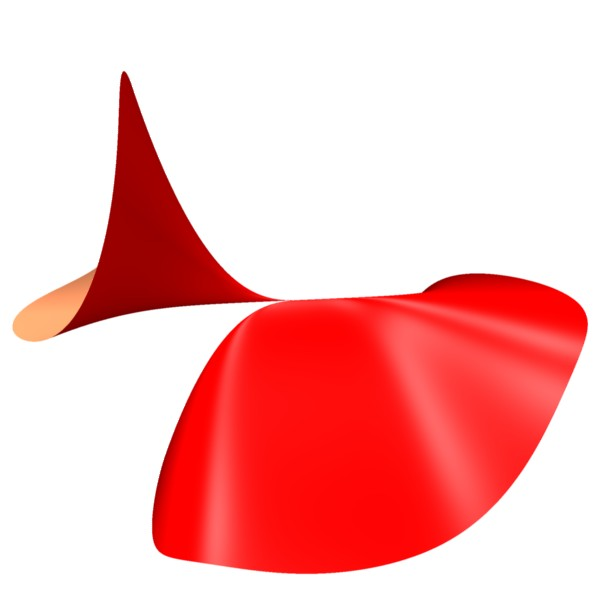
\includegraphics[width=1.2cm]{../../common/images/E8mm_0}
        \end{tabular}
        \end{tabular}
   \end{center}
    \vspace*{-0.4em}

An $E_8$ singularity may be deformed into a surface with seven real ordinary
double points by choosing $a$, $b$, and $c$ correctly in the following
family of equations: 
\[x\cdot((x-c)\cdot x-y\cdot (y-a)\cdot (y+a)\cdot(y-2b)\cdot(y+2b))-z^2=0\]

When choosing $c=1$ and varying $a$ and $b$, you will certainly be
able to find values for $a$ and $b$ such that the surface has seven
singularities (rightmost image).
We don't give a numerical solution here. 
Try to find one yourself!
    \begin{center}
      \begin{tabular}{@{}c@{\quad}c@{\quad}c@{}}
        \begin{tabular}{@{}c@{}}
          
\includegraphics[width=1.1cm]{../../common/images/E8mm_1}
        \end{tabular}
        &
        \begin{tabular}{@{}c@{}}
          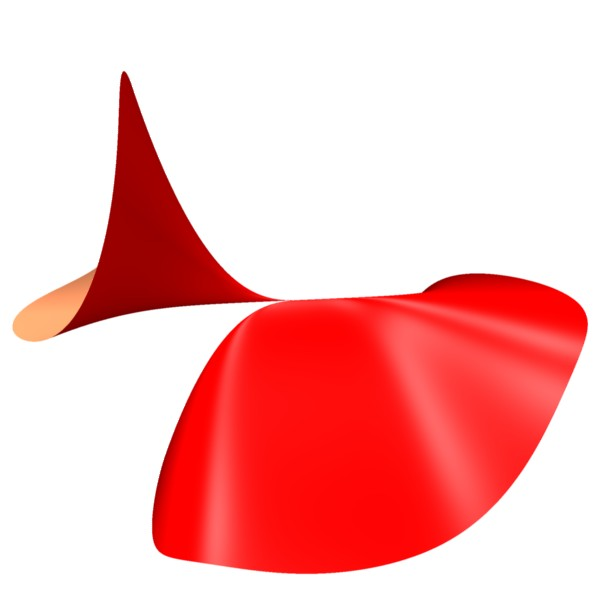
\includegraphics[width=1.1cm]{../../common/images/E8mm_0}
        \end{tabular}
        &
        \begin{tabular}{@{}c@{}}
          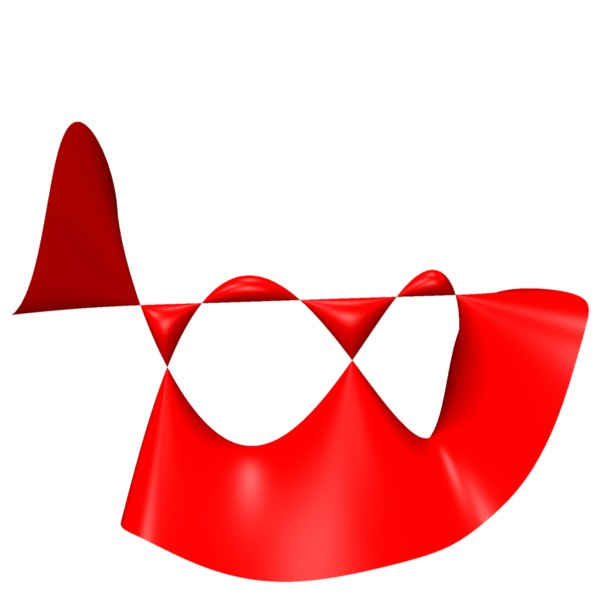
\includegraphics[width=1.1cm]{../../common/images/E8mm_2}
        \end{tabular}
     \end{tabular}
    \end{center}
\end{surferPage}
